\documentclass[final]{anthology-ch} % for the final version
%\documentclass{anthology-ch}         % for the submission

% LOAD LaTeX PACKAGES
\usepackage{booktabs}
\usepackage{graphicx}
\usepackage{tabularx}
\usepackage{minted}
\usemintedstyle{manni}
\usepackage{listings}
\usepackage{float}
\floatname{listing}{Listing}

% TITLE OF THE SUBMISSION
\title{There and back again---how to preserve your data during transformations}

% AUTHOR AND AFFILIATION INFORMATION
% For each author, include a new call to the \author command, with
% the numbers in brackets indicating the associated affiliations 
% (next section) and ORCID-ID for each author.  
\author[1]{Robert Casties}[
  orcid=0009-0008-9370-1303
]

% There should be one call to \affiliation for each affiliation of
% the authors. Multiple affiliations can be given to each author
% and an affiliation can be given to multiple authors. 
\affiliation{1}{Digital Humanities Team, Max Planck Institute for History of Science, Berlin, Germany}

% KEYWORDS
% Provide one or more keywords or key phrases seperated by commas
% using the following command
\keywords{software, best practice, data integrity, digital humanities}

% METADATA FOR THE PUBLICATION
% This will be filled in when the document is published; the values can
% be kept as their defaults when the file is submitted
\pubyear{2025}
\pubvolume{2}
\pagestart{6}
\pageend{12}
\conferencename{Digital Humanities Tech Symposium 2025}
\conferenceeditors{Julia Damerow and Rebecca Sutton Koeser}
\doi{10.63744/EZFV8PwG9Frz}  

\addbibresource{bibliography.bib}

%%%%%%%%%%%%%%%%%%%%%%%%%%%%%%%%%%%%%%%%%%%%%%%%%%%%%%%%%%%%%%%%%%%%%%%%%%%
% HERE IS THE START OF THE TEXT
\begin{document}

\maketitle

\begin{abstract}
Datasets often need to be transformed---from an external file format into a database, from one database system into another, or from an outdated legacy system into an archive format. All transformations carry the risk of data corruption through software errors. What can software developers do to check data integrity and make sure that data is not lost or changed in the process? This paper presents three basic approaches with different degrees of accuracy and complexity, illustrated by real-world examples. The first example shows simple end-to-end statistics by counting entities during the import of a dataset into a database, the next more complex example shows bookkeeping of entities during the conversion of an HTML website, and the last a full round-trip migration and comparison of a project database and data model.
\end{abstract}

\section{Introduction}

Digital Humanities projects work with many kinds of data. But the data is very rarely created, processed, visualized, backed up and archived in a single format in only one computer system. It is almost always transformed in one or more steps between formats and systems. The journey starts when data is loaded into a database from a source file in a structured format like XML, JSON, or CSV or an unstructured format like plain text. This process is also often called ETL (extract, transform, load). The journey continues when data is migrated from one database system to a different one or from one data model to another and it may end when the data is migrated into an archival format for long-term preservation or other data export formats for users to download and process. Each of these transformations carries the risk of inadvertent loss or corruption of data.

Most data transformations are done by software, often by multiple pieces of software by different authors. The integrity of transformed data depends therefore on the correctness of the software. The importance of software and of the correctness of software for the Digital Humanities has been argued more generally in  the context of improving software quality through code review \autocite{damerow_code_2025}. Code review and software tests as another element of good practice in software engineering often concentrate on small pieces of code and test small units with synthetic pieces of data. Software testing typically starts with isolated unit testing followed by more encompassing integration testing and system testing as described in an introductory text \autocite{leloudas_introduction_2023}. Testing data transformation integrity is not explicitly mentioned in this text, but it can be considered a type of end-to-end or system test where full, real input data is compared with the transformed output.

In the following, I present three basic methods that were applied in different projects to detect data loss and corruption in the data transformation process. The methods range from simple and easy to implement counting techniques to the development of rather complex and work-intensive re-transformation and comparison tools. The costs and benefits of applying each method have to be considered in the context of the specific project and development constraints, as in all software engineering decisions. The effort of considering and implementing measures to detect data loss and corruption was motivated by the need for insights into the migration process during the development cycle and by cases of real data loss in production.

\section{Forms of data loss and corruption}

Inadvertent changes to data can be categorized into basic categories:

\begin{itemize}
\item Entries are dropped (fewer than before)
\item Entries are added (more than before)
\item Entries are corrupted (same number but different content)
  \begin{itemize}
  \item Dropped, added, or corrupted attributes
  \item Dropped, added, or corrupted relations
  \end{itemize}
\end{itemize}

Depending on the system and data model, what is considered an entry can vary and attributes or relations of entities may not be strictly applicable. The concept of an entry being an entity with attributes that are simple data fields like strings or numbers and separate relations or references between entities works well for label-graph data models in graph databases like Neo4J or RDF and for object-oriented models in systems like Django\footnote{\url{https://docs.djangoproject.com/en/5.2/topics/db/models/}} that are translated into more elaborate relational database schemas behind the scenes. The concept does not necessarily apply to the transformation of HTML or XML. The basic categories of dropped, added, and corrupted entries apply more generally.

\section{Method 1: Count entities before and after transformation}

The simplest method is to count the entities in the data set before and after the transformation and to compare the counts. This method is easy to implement and able show data loss through dropped or added entities, but it cannot detect data corruption within the entities. Cases when an equal number of entities are added and dropped cannot be detected by this method. The impact of these issues can be reduced if groups of entities are counted and compared separately. In the example below, different types of entities are counted separately so that an added PLACE entity at the same time as a dropped PERSON entity would be detected even if the total number of entities stays the same.

An example for this method is the import process of an XML data file into a Drupal\footnote{\url{https://drupal.org/}} database. The project in question uses separate systems based on different technologies: a ResearchSpace\footnote{\url{https://researchspace.org/}} front end used by the domain experts for creating and editing the full dataset as CIDOC-CRM\footnote{\url{https://cidoc-crm.org/}} RDF data, and a Drupal website for the public presentation of the project results.

The ResearchSpace data curation interface creates a custom XML formatted data dump every night, which is imported into the Drupal website database. The import process is implemented using a bash script that extracts the entity count from the XML file for each entity type. In this case the script uses the existing \texttt{count} attribute in the custom XML format as seen in Listing~\ref{code:xml-fragment}, but it would also be possible to use an XML processor to count the relevant XML tags. After the import process the script runs a \texttt{drush} command to extract the count of Drupal entities of the same type using a custom view as seen in Listing~\ref{code:ismi-cnt} and compares the resulting numbers. The script then creates an error notification if the numbers for each entity type do not match.

\begin{listing}
\begin{minted}[fontsize=\small, highlightlines=2]{xml}
<openmind-data version="5.1">
  <entities count="300">
    <entity public="true" object-class="PLACE" id="1001961">Salähiyya madrasa
...
\end{minted}
 \caption{XML file fragment with entity count (top), and Drupal entity count command (bottom) for entities of type PLACE.}
\label{code:xml-fragment}
\end{listing}

\begin{listing}
\begin{minted}[fontsize=\small, highlightlines=3]{bash}
$ drush views:execute count_entities count_entities_csv place
count
300
\end{minted}
 \caption{drush command to extract the count of Drupal entities by type.}
\label{code:ismi-cnt}
\end{listing}

\section{Method 2: Keep track of entities during transformation steps}

An intermediate method is internal bookkeeping in a transformation script. It is often possible to create counts and lists of items as they are read and compare these numbers or lists to the results of later stages of the transformation process. This method can detect dropped or added entities and, depending on the implementation, also some cases of corrupted entities. If items can be individually identified and kept in lists or sets it is possible to differentiate between added and dropped items and identify which items were added or dropped even if the total count stays the same.

An example is a migration script that processes hundreds of HTML files that are the result of web scraping and a separate JSON file containing the navigation hierarchy exported from a dynamic legacy Zope\footnote{\url{https://www.zope.dev/}} website. The migration script uses the HTML and JSON input files to create a corrected static HTML website. The script reads the navigation hierarchy file and the raw HTML files and processes the HTML by comparing links to other HTML files within the navigation hierarchy data to create correct links, omit duplicated files, and find broken links.

\begin{listing}
\begin{minted}[fontsize=\footnotesize, highlightlines={4,20}]{python}
# check all links
links = set()
nav_path = nav_item['echo_path']
for atag in soup.find_all('a'):
    if 'href' in atag.attrs:
        link = atag['href'].strip()
...
        # process interactive map links
        if 'onmouseover' in atag.attrs:
            # get linked item from id
            m = maplink_id_pattern.match(atag['id'])
            if m:
                nav_link = nav_path + '/' + m.group(1).replace(' ', '%20')
                if nav_link in args.nav_struct:
                    link_item = args.nav_struct[nav_link]
                    if link_item['type'] == 'ECHO_resource':
                        if 'link' in link_item and 'digilib.html?' in link_item['link']:
                            # replace link to ECHO_resource linking to digilib
                            atag['href'] = link_item['link']
                            processed_items.add(nav_link)
                            continue
...                        
        # add to be processed later
        links.add(link)
\end{minted}

\caption{Python script fragment showing a loop processing all a tags in an HTML document and adding a processed item.}
  \label{code:echo-loop}
\end{listing}

During the process the script keeps a list of processed HTML files, and the links in each file, indexed by URL, as a Python set. Listing~\ref{code:echo-loop} shows a part of the main loop running through all HTML \texttt{a} tags representing links in a document, fixing the links and adding the successfully processed links to the set of processed links.

\begin{listing}
\begin{minted}[fontsize=\footnotesize, highlightlines={2,13}]{python}
# initialize processed_items with ignore_items
args.processed_items = set(args.ignore_items)

args.processed_files = set()
# process files starting at index page
start_file = args.echo_section + '/index.html'
logging.info(f"start processing at {start_file}")
start_file = args.html_files[start_file]
# process files (modifies args.processed_items and args.processed_files)
process_files(start_file, in_path, out_path, args)
...
# check number of unprocessed items
unprocessed_items = set(args.nav_struct.keys()) - args.processed_items
\end{minted}
  \caption{Python script fragment with a highlighted set of processed items and set math to determine unprocessed items.}
  \label{code:echo-tracking}
\end{listing}

This makes it possible to compare the number of processed items to the expected total based on the navigation hierarchy data. Since files and links are identified by URL, processed links can be removed from the expected links in the navigation hierarchy using set operations to generate the set of unprocessed items, as shown in Listing~\ref{code:echo-tracking}. This method can therefore also show errors in cases where an HTML file name or link is different from the navigation structure URL, which a simple count would not reveal.

\section{Method 3: Round-trip entities and compare to the source format}

The most comprehensive and also most time-consuming strategy to test a transformation from one format into another is the development and application of an inverse transformation that converts the result format back into the source format and allows to compare the result to the original dataset in the original format. This method is the most comprehensive because it allows to check for data corruption in the entities as well as for data loss. The method is also time-consuming because it requires the development of an additional transformation step that can be similarly complex to the original transformation.

An example for this case is the migration of the ISMI\footnote{\url{https://ismi.mpiwg-berlin.mpg.de}} project database from a legacy custom database software called OpenMind using a label-graph data model into a standard CIDOC-CRM based data model in RDF with a ResearchSpace front end. The biggest challenges in developing and testing this transformation were differences in the data models. The original label-graph data model consisted of about 40,000 nodes of 18 types with 60,000 relations whereas the resulting CIDOC-CRM data model consisted of about 900,000 RDF triples of 100 ontology classes. In the label-graph model a node of type \texttt{person} has an attribute \texttt{name} containing the name as a string while in the CIDOC-CRM model a Person URI has a relation to an Appellation URI that has a relation to a Literal containing the name. There are additional differences between the old data model and the new standard model that required multiple entities for each text and witness entity in the new FRBRoo-based\footnote{\url{https://cidoc-crm.org/frbroo/}} model.

The original migration from OpenMind to CIDOC-CRM used the X3ML\footnote{\url{https://github.com/isl/x3ml}} tool and language to create RDF. To check the results of this transformation, I developed an additional transformation from RDF back into the original OpenMind data model and a comparison tool to show differences in the resulting data sets using Python. Figure~\ref{fig:ismi-round-trip} shows a diagram of the full process.

The ability to run this test was an invaluable asset during the development of the migration mapping. It allowed to find bugs in the initial mapping and to refactor the mapping incrementally to better align with requirements of the ResearchSpace front end, in the knowledge that any data corruption in the process would become immediately visible. The functional role that tests can have during software development is emphasized even more in methods like Test Driven Development (TDD).

\begin{figure}[]
  \centering
  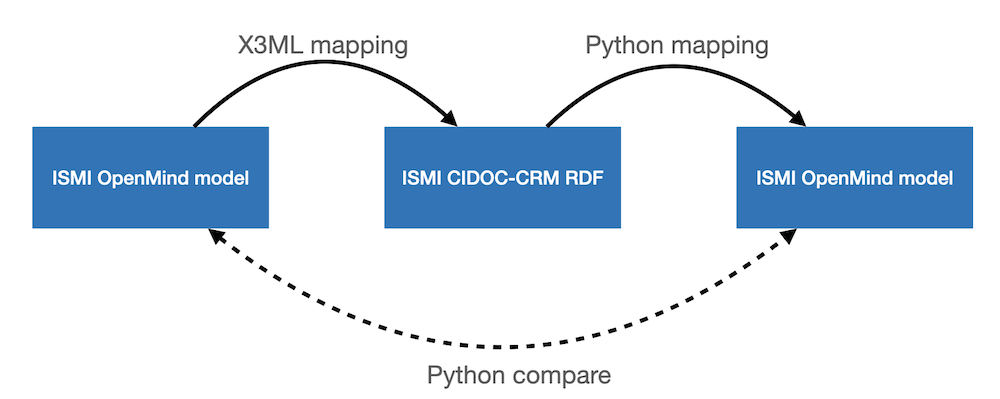
\includegraphics[width=0.8\linewidth]{figures/ismi-round-trip.png}
  \caption{Round-trip migration from the old OpenMind database model via a X3ML mapping to the new CIDOC-CRM RDF database model and back into the OpenMind model through a Python mapping allowing a Python comparison tool to test the result in the same kind of model.}
  \label{fig:ismi-round-trip}
\end{figure}

The comparison tool has options to selectively enable or disable certain checks or exclude specific relation, attribute, or entity types as shown in Listing~\ref{code:ismi-compare}. These options were used during the development process to focus on specific areas of the transformation in order to not drown in thousands of unrelated error messages, particularly during the early phase of development. Watching the number of errors go down was also a satisfying measure of development progress.

\begin{listing}
\begin{minted}[fontsize=\scriptsize]{text}
usage: compare_models.py [-h] [--version] [--ignore-nodes IGNORE_NODES]
                         [--ignore-attributes IGNORE_ATTRIBUTES]
                         [--ignore-relations IGNORE_RELATIONS] [--show-nodes] [--show-relations]
                         [--show-attributes] [--check-attribute-content] [-l {INFO,DEBUG,ERROR}]
                         file1 file2

Compare two networkx graphs with ISMI data.

positional arguments:
  file1                 First networkx graph in gpickle format
  file2                 Second networkx graph in gpickle format

options:
  -h, --help            show this help message and exit
  --version             show program's version number and exit
  --ignore-nodes IGNORE_NODES
                        list of node types to ignore (comma-separated)
  --ignore-attributes IGNORE_ATTRIBUTES
                        list of attributes to ignore on all entities (comma-separated)
  --ignore-relations IGNORE_RELATIONS
                        list of relations to ignore on all entities (comma-separated)
  --show-nodes          show node differences in detail
  --show-relations      show relation differences in detail
  --show-attributes     show attribute differences in detail
  --check-attribute-content
                        check attribute content (optional)
\end{minted}
  \caption{Command line options for the Python model comparison tool compare\_models, including options to show more or less detailed differences or to ignore specific item, attribute, or relation types.}
  \label{code:ismi-compare}
\end{listing}


\section{Conclusion}

The three basic methods for testing data integrity presented here have different strengths and weaknesses and every developer needs to weigh these against the requirements of the individual project and the available development resources. Table~\ref{tab:method-abilities} shows an overview of the methods and their ability to detect dropped or added or corrupted entities versus the implementation complexity.

\begin{table}[h]
  \centering
  \begin{tabular}{>{\raggedright}p{0.3\textwidth} >{\centering}p{0.2\textwidth} >{\centering}p{0.2\textwidth} c}
    Method & Detect dropped or added entities & Detect corrupted entities & Complexity \\ \midrule
    1: Count entities before and after transformation & yes (if total number changes) & no & low \\ \midrule
    2: Keep track of entities during transformation & yes & possible & medium \\ \midrule
    3: Round-trip entities and compare result & yes & yes & high \\ \bottomrule
  \end{tabular}
  \caption{Detection abilities and complexity cost of three methods.}
  \label{tab:method-abilities}
\end{table}

Creating and running different kinds of tests has become an integral part of good practice of software development in general. Tests let you trust your own code during and after active development. Tests also let others that review or use your code, trust the code. Tests can also be an active part of the development process when they allow to measure progress during the early phases of development or when they help to detect and avoid regressions when refactoring the code. The basic methods of end-to-end testing of data integrity shown here can be part of every developer's toolbox of tests to apply, depending on the requirements of the development project.

Another good practice of software development is the sharing of code in---preferably public---repositories to enable code review, re-use, or just the sharing of programming techniques and ideas. The repositories containing the scripts used as examples for methods 1 and 2 are not publicly available, but the scripts used for method~3 are available as part of the ISMI data model repository.\footnote{\url{https://gitlab.gwdg.de/MPIWG/Department-II/ismi-cidoc-model/-/tree/master/Tools/graph-tools}}


% Print the biblography at the end. Keep this line after the main text of your paper, and before an appendix. 
\printbibliography

% You can include an appendix using the following command
%\appendix

\end{document}
